% !TEX program = xelatex
\documentclass[12pt, a4paper, oneside]{book}
% !TEX root = ../do-an.tex
% =====================================================================
%  styles/settings.tex
%  Các thiết lập chung, nạp từ file chính do-an.tex.
%  SINH VIÊN KHÔNG SỬA FILE NÀY.
%
%  Lưu ý: lệnh khai báo lớp tài liệu nằm ở file do-an.tex chứ không nằm
%  ở đây. Lý do: Overleaf dò file chính bằng cách tìm chuỗi khai báo lớp
%  tài liệu trong các file. Nếu chuỗi đó xuất hiện ở file này, Overleaf
%  sẽ biên dịch nhầm file này và báo lỗi "no legal end found", vì file
%  này chỉ chứa thiết lập chứ không chứa phần thân tài liệu.
% =====================================================================

% Toàn bộ nhận diện DAU: phông, màu, bìa, hộp trình bày, header
\usepackage{styles/dau}
\dauLayout

% Giãn dòng và khoảng cách đoạn theo quy cách đồ án
\linespread{1.25}
\usepackage[skip=8pt plus 1pt, indent=15pt]{parskip}

% Ghi chú: mẫu gốc dùng gói atbegshi để vứt trang đầu, vì trang bìa của
% mẫu gốc dựng bằng minipage nên sinh ra một trang trắng. Trang bìa ở
% đây dựng bằng môi trường titlepage nên không có trang trắng, và nếu
% giữ thủ thuật đó thì chính trang bìa sẽ bị vứt mất.


\crname{BÁO CÁO ĐỒ ÁN TRÍ TUỆ NHÂN TẠO}
\cmonhoc{Học phần AIP202 \textperiodcentered{} 2 tín chỉ}
\ctname{XÂY DỰNG TRỢ LÝ TUYỂN DỤNG\\ỨNG DỤNG TRÍ TUỆ NHÂN TẠO}
\cstuname{[Họ và tên sinh viên]}
\cmssv{[Mã số sinh viên]}
\clopsv{[Lớp]}
\csCouncil{Công nghệ thông tin}
\csSupervise{[Tên giảng viên hướng dẫn]}
\cttime{[Năm học]}
\csdeptname{KHOA CÔNG NGHỆ THÔNG TIN}
\csplace{Đà Nẵng}

\begin{document}
\coverpage
\frontmatter
\dauPageStyle
\begin{declaration}

\textit{[Sinh viên đọc kỹ nội dung cam đoan, xác nhận tính chính xác và ký trước khi nộp.]}

Tôi xin cam đoan đồ án ``Xây dựng trợ lý tuyển dụng ứng dụng trí tuệ nhân tạo'' là công trình do chính tôi thực hiện dưới sự hướng dẫn của \dauGVHD. Các nội dung nghiên cứu, số liệu và kết quả trình bày trong đồ án là trung thực trong phạm vi dữ liệu và quá trình thực hiện được mô tả trong báo cáo.

Mọi tài liệu, hình ảnh, mã nguồn và kết quả của tác giả khác được sử dụng trong đồ án đều được trích dẫn nguồn gốc rõ ràng. Những phần có sử dụng công cụ trí tuệ nhân tạo hỗ trợ được khai báo theo quy định của học phần và Nhà trường.

\vspace{1.4em}
\hfill\okyten{\dauSinhVien}{Sinh viên thực hiện}

\end{declaration}

\begin{acknowledgments}

\textit{[Bản nháp: cá nhân hóa lời cảm ơn và xác nhận những người/đơn vị thực tế đã hỗ trợ trước khi nộp.]}

Em xin chân thành cảm ơn giảng viên hướng dẫn đã định hướng và góp ý trong quá trình thực hiện đồ án. Em xin cảm ơn quý thầy cô Khoa Công nghệ Thông tin, Trường Đại học Kiến trúc Đà Nẵng đã trang bị kiến thức nền tảng cho em. Em cũng xin cảm ơn gia đình và bạn bè đã động viên em trong quá trình học tập và hoàn thành đồ án.

\vspace{1.4em}
\hfill\okyten{\dauSinhVien}{Sinh viên thực hiện}

\end{acknowledgments}

\begin{abstract}

Đồ án xây dựng một ứng dụng hỗ trợ quy trình tuyển dụng gồm quản lý vị trí tuyển dụng và hồ sơ ứng viên, đọc thông tin từ CV, so khớp ứng viên với công việc và cung cấp giao diện theo dõi cho nhà tuyển dụng. Hệ thống có giao diện React/Vite gọi API FastAPI; dữ liệu phát triển được lưu bằng SQLite. Bộ đọc hồ sơ tiếp nhận PDF và DOCX, trích xuất văn bản và nhận diện một số trường phổ biến. Với PDF scan, hệ thống có nhánh OCR dự phòng phụ thuộc Tesseract và dữ liệu ngôn ngữ được cài đặt.

Phần so khớp kết hợp kỹ năng, kinh nghiệm, học vấn, dự án và tương đồng nội dung. Đồ án cũng huấn luyện mô hình Random Forest phân loại mức độ phù hợp. Trên tập kiểm thử được tách theo hồ sơ ứng viên, mô hình đạt accuracy 0,7128 và macro F1 0,5645; baseline dự đoán lớp phổ biến đạt accuracy 0,7434 và macro F1 0,2843. Như vậy, mô hình có macro F1 cao hơn nhưng accuracy thấp hơn baseline. Dữ liệu đánh giá có thành phần tổng hợp và nhãn được hỗ trợ bằng mô hình, nên kết quả chỉ mang ý nghĩa thử nghiệm, chưa đại diện cho hiệu quả tuyển dụng thực tế. Hệ thống được định hướng như công cụ hỗ trợ rà soát; người tuyển dụng cần kiểm tra thông tin và tự đưa ra quyết định.

\vspace{0.8em}
\noindent\textbf{Từ khoá:} tuyển dụng, phân tích CV, trích xuất thông tin, so khớp ứng viên, Random Forest.

\end{abstract}

\tableofcontents
\listoffigures
\listoftables
\mainmatter
\dauPageStyle
\chapter{Mở đầu}
\label{ch:modau}

\begin{muctieu}
Chương này trình bày bối cảnh, mục tiêu, phạm vi và bố cục của đồ án xây dựng trợ lý tuyển dụng.
\end{muctieu}

\section{Lý do chọn đề tài}
Quy trình tuyển dụng thường phải xử lý nhiều CV với định dạng và cách trình bày khác nhau. Việc nhập lại thông tin, đối chiếu từng hồ sơ với yêu cầu công việc và theo dõi trạng thái ứng viên có thể tốn thời gian. Nghiên cứu về trích xuất thông tin CV cũng chỉ ra rằng sự đa dạng về bố cục gây khó khăn cho khai phá thông tin, so khớp công việc và xếp hạng ứng viên~\cite{Chen2018,Palshikar2023}.

Đồ án chọn bài toán xây dựng trợ lý tuyển dụng để kết hợp quản lý dữ liệu với trích xuất văn bản và xếp hạng ứng viên. Hệ thống được định hướng là công cụ hỗ trợ người tuyển dụng: thông tin trích xuất cần được đối chiếu với CV gốc, còn quyết định tuyển dụng do con người đưa ra.

\section{Mục tiêu của đồ án}
Đồ án hướng tới các mục tiêu sau:
\begin{itemize}[leftmargin=1.6em,itemsep=2pt]
  \item Xây dựng giao diện quản lý vị trí tuyển dụng, ứng viên, CV và kết quả so khớp.
  \item Tiếp nhận PDF/DOCX và trích xuất văn bản cùng một số trường thông tin phổ biến.
  \item Tính điểm so khớp theo nhiều tiêu chí và trình bày được các tín hiệu chính.
  \item Thử nghiệm mô hình phân loại mức độ phù hợp, đánh giá trên tập dữ liệu tách theo hồ sơ ứng viên.
  \item Đóng gói môi trường phát triển bằng Docker Compose và cung cấp API cho giao diện.
\end{itemize}

\section{Phạm vi và đối tượng}
Đối tượng sử dụng hướng tới là nhà tuyển dụng hoặc người quản lý quy trình tuyển dụng trong môi trường thử nghiệm. Phạm vi hiện tại tập trung vào CV PDF/DOCX, các trường văn bản phổ biến và một số nhóm tiêu chí so khớp. Độ chính xác phụ thuộc cấu trúc CV, chất lượng văn bản/OCR, từ điển kỹ năng và dữ liệu huấn luyện.

Bộ dữ liệu đánh giá hiện có 93.733 bản ghi từ 643 hồ sơ ứng viên và 351 mô tả công việc. Dữ liệu có thành phần tổng hợp và nhãn được hỗ trợ bằng mô hình, nên không được xem là benchmark độc lập do con người gán nhãn. Kết quả chỉ dùng để thử nghiệm kỹ thuật trong phạm vi đồ án.

\section{Bố cục báo cáo}
Chương~\ref{ch:coso} trình bày cơ sở lý thuyết, công nghệ và nghiên cứu liên quan. Chương~\ref{ch:thietke} phân tích yêu cầu, kiến trúc, dữ liệu và thuật toán. Chương~\ref{ch:caidat} mô tả cài đặt, tích hợp và kiểm tra phần mềm. Chương~\ref{ch:ketqua} trình bày kết quả đánh giá và hạn chế. Chương~\ref{ch:ketluan} tổng kết và nêu hướng phát triển.

\chapter{Cơ sở lý thuyết và công nghệ}
\label{ch:coso}

\begin{muctieu}
Chương này giới thiệu các nền tảng trực tiếp được sử dụng trong bộ đọc CV, thuật toán so khớp, mô hình phân loại và ứng dụng web.
\end{muctieu}

\section{Kiến thức nền tảng}
\subsection{Trích xuất văn bản từ CV}
PDF có thể chứa lớp văn bản hoặc chỉ có ảnh quét. Hệ thống dùng bộ trích xuất PDF cho nội dung văn bản; với trang có ít văn bản hoặc lớp chữ mỏng trên nền scan, mã nguồn có thể kết xuất trang và thử OCR. DOCX được đọc từ các đoạn văn bản, bảng, đầu trang và chân trang. OCR phụ thuộc cài đặt Tesseract cùng dữ liệu ngôn ngữ tiếng Anh và tiếng Việt. Kết quả trích xuất không đảm bảo giữ nguyên thứ tự đọc của bố cục nhiều cột hoặc nội dung trong ảnh.

Sau khi đọc tệp, bộ phân tích dò thông tin liên hệ, kỹ năng, học vấn và kinh nghiệm. Mốc năm trong phần học vấn có thể bị nhầm thành kinh nghiệm nếu chỉ dựa vào biểu thức thời gian; vì vậy ngữ cảnh tiêu đề và đoạn văn cần được xem xét. Các trường trích xuất phải cho phép người dùng kiểm tra và sửa.

\subsection{TF-IDF và độ tương đồng cosine}
TF-IDF biểu diễn văn bản bằng trọng số từ, giảm ảnh hưởng của từ xuất hiện phổ biến trong nhiều tài liệu. Khi CV và mô tả công việc được chuyển thành vector, độ tương đồng cosine được tính bằng tích vô hướng đã chuẩn hóa:
\begin{equation}
\operatorname{cos}(x,y)=\frac{x\cdot y}{\lVert x\rVert\lVert y\rVert}.
\end{equation}
Đây là tín hiệu tương đồng từ vựng gọn nhẹ, nhưng có thể bỏ sót từ đồng nghĩa nếu không có chuẩn hóa hoặc mô hình ngữ nghĩa~\cite{Manning2008}.

\subsection{Embedding ngữ nghĩa}
Embedding ánh xạ văn bản thành vector để so sánh ngữ nghĩa. Trong dự án, embedding là cấu hình tùy chọn; khi nhà cung cấp embedding không khả dụng, matching dùng TF-IDF. Báo cáo đánh giá hiện có ghi semantic model không khả dụng, nên kết quả thực nghiệm không được diễn giải như đánh giá của embedding.

\subsection{Random Forest và độ đo}
Random Forest kết hợp nhiều cây quyết định được huấn luyện trên các mẫu và đặc trưng khác nhau~\cite{Breiman2001}. Accuracy đo tỷ lệ dự đoán đúng tổng thể. Macro F1 lấy trung bình F1 của từng lớp với trọng số bằng nhau, do đó hữu ích khi phân bố lớp không cân bằng. Các chỉ số phụ thuộc cách chia dữ liệu và chất lượng nhãn.

\section{Công cụ và thư viện}
\begin{table}[H]
\centering
\caption{Các công nghệ chính được sử dụng trong dự án.}
\label{tab:congcu}
\begin{tabular}{p{0.25\textwidth}p{0.33\textwidth}p{0.34\textwidth}}
\toprule
\textbf{Thành phần} & \textbf{Công nghệ} & \textbf{Vai trò} \\
\midrule
Giao diện & React, Vite, React Router, Axios & Hiển thị trang và gọi API \\
API & FastAPI, Pydantic & Endpoint và kiểm tra dữ liệu \\
Truy cập dữ liệu & SQLAlchemy, SQLite & Ánh xạ mô hình và lưu dữ liệu phát triển \\
Đọc CV & pdfplumber, PyMuPDF, python-docx, Tesseract tùy chọn & Đọc PDF/DOCX và OCR dự phòng \\
Học máy & scikit-learn & TF-IDF, Random Forest và đánh giá \\
Đóng gói & Docker Compose & Khởi chạy frontend và backend \\
\bottomrule
\end{tabular}
\end{table}

Trong cấu hình phát triển, Compose công bố frontend ở cổng 5173 và API ở cổng 8000. \code{0.0.0.0} là địa chỉ bind trong dịch vụ; khi truy cập trên máy host, dùng \url{http://localhost:5173} cho giao diện và \url{http://localhost:8000/docs} cho tài liệu API.

\section{Các công trình liên quan}
Các nghiên cứu trích xuất CV xem hồ sơ là tài liệu bán cấu trúc, trong đó thông tin thường được chia thành các khối như liên hệ, học vấn và kinh nghiệm. Chen và cộng sự đề xuất quy trình hai bước: phân đoạn khối nội dung trước, sau đó nhận diện các thuộc tính chi tiết~\cite{Chen2018}. Hệ thống RINX kết hợp mẫu ngôn ngữ, từ điển và kỹ thuật học máy để trích xuất thông tin từ hồ sơ dạng tự do~\cite{Palshikar2023}. Các hướng này cho thấy việc giữ ngữ cảnh khối có ích hơn việc tìm chuỗi độc lập, nhưng chất lượng vẫn phụ thuộc ngôn ngữ và định dạng dữ liệu.

Trong phạm vi đồ án, bộ đọc dùng trích xuất PDF/DOCX và các quy tắc nhận diện trường; chưa triển khai mô hình phân đoạn CV huấn luyện chuyên biệt. Các tổng quan về công bằng trong tuyển dụng thuật toán nhấn mạnh rằng hệ thống xếp hạng cần được đánh giá về thiên lệch, dữ liệu và tác động lên các nhóm ứng viên~\cite{Fabris2025}. Vì vậy, điểm so khớp trong đồ án chỉ hỗ trợ rà soát, không nên là căn cứ duy nhất để ra quyết định.


\chapter{Phân tích và thiết kế}
\label{ch:thietke}

\begin{muctieu}
Chương này phân tích yêu cầu bài toán, kiến trúc ứng dụng, mô hình dữ liệu, bộ trích xuất CV, điểm so khớp và pipeline phân loại.
\end{muctieu}

\section{Phân tích bài toán và yêu cầu}
Quy trình sử dụng gồm: nhà tuyển dụng đăng nhập; tạo vị trí cùng mô tả và tiêu chí; tải CV lên; kiểm tra hồ sơ đã trích xuất; sau đó xem kết quả so khớp và thông tin giải thích. Hệ thống cần giữ liên kết giữa tệp CV, ứng viên, vị trí và kết quả để người dùng có thể truy vết.

Yêu cầu chức năng chính gồm xác thực người dùng; quản lý vị trí; tải CV; trích xuất và lưu hồ sơ ứng viên; tính điểm phù hợp; lưu kết quả và cung cấp số liệu tổng quan. Yêu cầu phi chức năng gồm báo rõ trạng thái tải tệp/lỗi API, kiểm tra loại tệp, bảo vệ token và dữ liệu cá nhân, cùng khả năng người dùng rà soát kết quả tự động.

\section{Thiết kế kiến trúc hệ thống}
Hình~\ref{fig:kientruc} khái quát luồng xử lý từ giao diện đến các dịch vụ backend. Giao diện React/Vite gọi API FastAPI; backend xác thực yêu cầu, điều phối đọc CV, matching và truy cập cơ sở dữ liệu thông qua SQLAlchemy.

\begin{figure}[H]
\centering
\resizebox{\textwidth}{!}{%
\begin{tikzpicture}[node distance=10mm and 11mm]
  \node[objbox] (user) {Nhà tuyển dụng};
  \node[clsbox, right=of user] (web) {React / Vite\\Giao diện};
  \node[clsbox, right=of web] (api) {FastAPI\\REST API};
  \node[clsbox, above right=of api] (db) {SQLAlchemy\\SQLite};
  \node[objbox, below right=of api] (file) {PDF / DOCX};
  \node[clsbox, right=of file] (parse) {Trích xuất\\OCR tùy chọn};
  \node[clsbox, right=of parse] (match) {Matching\\Random Forest};
  \draw[flowarr] (user) -- (web);
  \draw[flowarr] (web) -- (api);
  \draw[flowarr] (api) -- (db);
  \draw[flowarr] (api) -- (file);
  \draw[flowarr] (file) -- (parse);
  \draw[flowarr] (parse) -- (match);
  \draw[flowarr] (match) |- (api);
\end{tikzpicture}}
\caption{Kiến trúc khái quát của trợ lý tuyển dụng.}
\label{fig:kientruc}
\end{figure}

Các router backend được chia theo miền xác thực, vị trí, ứng viên, CV, matching, dashboard và trạng thái mô hình. SQLite là cấu hình cơ sở dữ liệu phát triển; tệp CV được lưu trên vùng uploads của backend.

\section{Thiết kế dữ liệu}
Các thực thể chính trong mã nguồn gồm người dùng, vị trí, ứng viên, CV, kết quả so khớp, chi tiết so khớp, kỹ năng và nhật ký phân tích. Mỗi ứng viên có thể liên kết nhiều tệp CV; mỗi kết quả so khớp tham chiếu một vị trí và một ứng viên. Bảng~\ref{tab:thucthe} tóm tắt một số trường tiêu biểu; cấu trúc chi tiết nằm trong các model SQLAlchemy.

\begin{table}[H]
\centering
\caption{Một số thực thể và dữ liệu được lưu.}
\label{tab:thucthe}
\begin{tabular}{p{0.22\textwidth}p{0.69\textwidth}}
\toprule
\textbf{Thực thể} & \textbf{Dữ liệu tiêu biểu} \\
\midrule
User & Tên, email, mật khẩu băm, vai trò \\
Job & Tiêu đề, mô tả, trạng thái, kỹ năng yêu cầu, kinh nghiệm và học vấn yêu cầu \\
Candidate & Thông tin liên hệ, tóm tắt, văn bản gốc, kỹ năng, học vấn, kinh nghiệm, dự án, chứng chỉ và ngôn ngữ \\
Resume & Tên/đường dẫn tệp, văn bản trích xuất, trạng thái và phiên bản phân tích \\
Match & Điểm tổng, điểm thành phần, lớp dự đoán, độ tin cậy và snapshot đặc trưng \\
MatchDetail & Kỹ năng, loại khớp, điểm, trạng thái và mô tả \\
\bottomrule
\end{tabular}
\end{table}

\section{Thiết kế mô hình và thuật toán}
\subsection{Bộ phân tích CV}
Luồng đọc tệp gồm kiểm tra phần mở rộng, trích xuất nội dung PDF/DOCX, chuẩn hóa văn bản, nhận diện trường và lưu hồ sơ. PDF được thử trích xuất lớp chữ bằng pdfplumber; nếu nội dung quá ngắn hoặc trang có ảnh scan lớn, PyMuPDF kết xuất trang để Tesseract OCR thử đọc bằng ngôn ngữ \code{eng+vie}. DOCX được đọc từ đoạn văn, bảng, đầu trang và chân trang.

Các trường mục tiêu gồm thông tin liên hệ, kỹ năng, học vấn, kinh nghiệm, dự án, chứng chỉ và ngôn ngữ. OCR và quy tắc dò trường có thể sai với bố cục phức tạp. Một số nhận diện thời gian dựa trên chuỗi năm/tháng nên cần rà soát ngữ cảnh để không tính thời gian học thành kinh nghiệm làm việc.

\subsection{Điểm so khớp ứng viên}
Mã nguồn kết hợp điểm kỹ năng, kinh nghiệm, học vấn, dự án và tương đồng nội dung. Trọng số hiện cài đặt được trình bày ở Bảng~\ref{tab:trongso}. Điểm kỹ năng dựa trên tỷ lệ kỹ năng bắt buộc đã khớp; kinh nghiệm đối chiếu số năm; học vấn dùng cấp độ nhận diện; điểm dự án hiện là heuristic dựa trên cụm từ; tương đồng nội dung dùng TF-IDF và cosine similarity.

\begin{table}[H]
\centering
\caption{Trọng số các thành phần của điểm so khớp.}
\label{tab:trongso}
\begin{tabular}{lr}
\toprule
\textbf{Thành phần} & \textbf{Trọng số} \\
\midrule
Kỹ năng & 40\% \\
Kinh nghiệm & 15\% \\
Học vấn & 15\% \\
Dự án & 10\% \\
Tương đồng nội dung & 20\% \\
\bottomrule
\end{tabular}
\end{table}

Khi embedding sentence-transformer khả dụng, phần tương đồng nội dung chia thành TF-IDF 10\% và semantic similarity 10\%; khi không khả dụng, TF-IDF chiếm 20\%. Đây là trọng số cấu hình trong mã, không phải tham số được tối ưu qua nghiên cứu người dùng.

\subsection{Mô hình phân loại}
Pipeline huấn luyện sử dụng Random Forest với cân bằng lớp và \code{random\_state=42}. Tập dữ liệu có 93.733 bản ghi, 643 hồ sơ CV duy nhất và 351 mô tả công việc. Dữ liệu được chia theo nhóm hồ sơ ứng viên thành 65.419 mẫu huấn luyện, 14.386 mẫu validation và 13.928 mẫu kiểm thử. Cách chia nhóm hạn chế một ứng viên xuất hiện ở nhiều tập, nhưng không loại bỏ việc nội dung mô tả công việc có thể lặp giữa các tập.

\chapter{Cài đặt và thử nghiệm}
\label{ch:caidat}

\begin{muctieu}
Chương này trình bày môi trường phát triển, cách tích hợp các thành phần, giao diện và trạng thái kiểm tra phần mềm.
\end{muctieu}

\section{Môi trường triển khai}
Dự án gồm frontend React/Vite và backend FastAPI. Docker Compose cấu hình frontend tại cổng 5173, backend tại cổng 8000, SQLite trong backend và thư mục uploads để lưu tệp. Có thể truy cập giao diện bằng \url{http://localhost:5173} và tài liệu API bằng \url{http://localhost:8000/docs}. Địa chỉ \code{0.0.0.0} dùng để dịch vụ lắng nghe kết nối bên trong môi trường chạy, không phải URL người dùng nhập vào trình duyệt.

Bộ đọc OCR phụ thuộc Tesseract và dữ liệu ngôn ngữ. Trong cấu hình Docker dự án, các thành phần OCR được cài trong image backend; khi chạy trực tiếp trên Windows, cần cài Tesseract cùng dữ liệu Anh/Việt theo README. Phiên bản phần mềm và cấu hình máy dùng để chạy lần cuối cần được bổ sung trước khi nộp.

\section{Các thành phần chính}
Frontend gọi API theo các miền chức năng và hiển thị trạng thái tải, lỗi hoặc kết quả. Backend dùng các router riêng để xử lý xác thực, vị trí, ứng viên/CV, matching, dashboard và model. Bộ phân tích CV tạo văn bản trích xuất và dữ liệu ứng viên; MatchingEngine tính các điểm tiêu chí và trả về giải thích cùng các kỹ năng đã khớp/thiếu. Pipeline Random Forest là một nhánh dự đoán riêng; API có thể trả chế độ fallback khi artifact mô hình chưa được nạp.

\section{Giao diện và demo}
Hình~\ref{fig:cvreview} là ảnh giao diện xem lại một CV minh họa, dùng để quan sát cấu trúc thông tin sau phân tích. Nội dung hồ sơ trong ảnh là dữ liệu mẫu, không phải hồ sơ người dùng thật.

\begin{figure}[H]
\centering
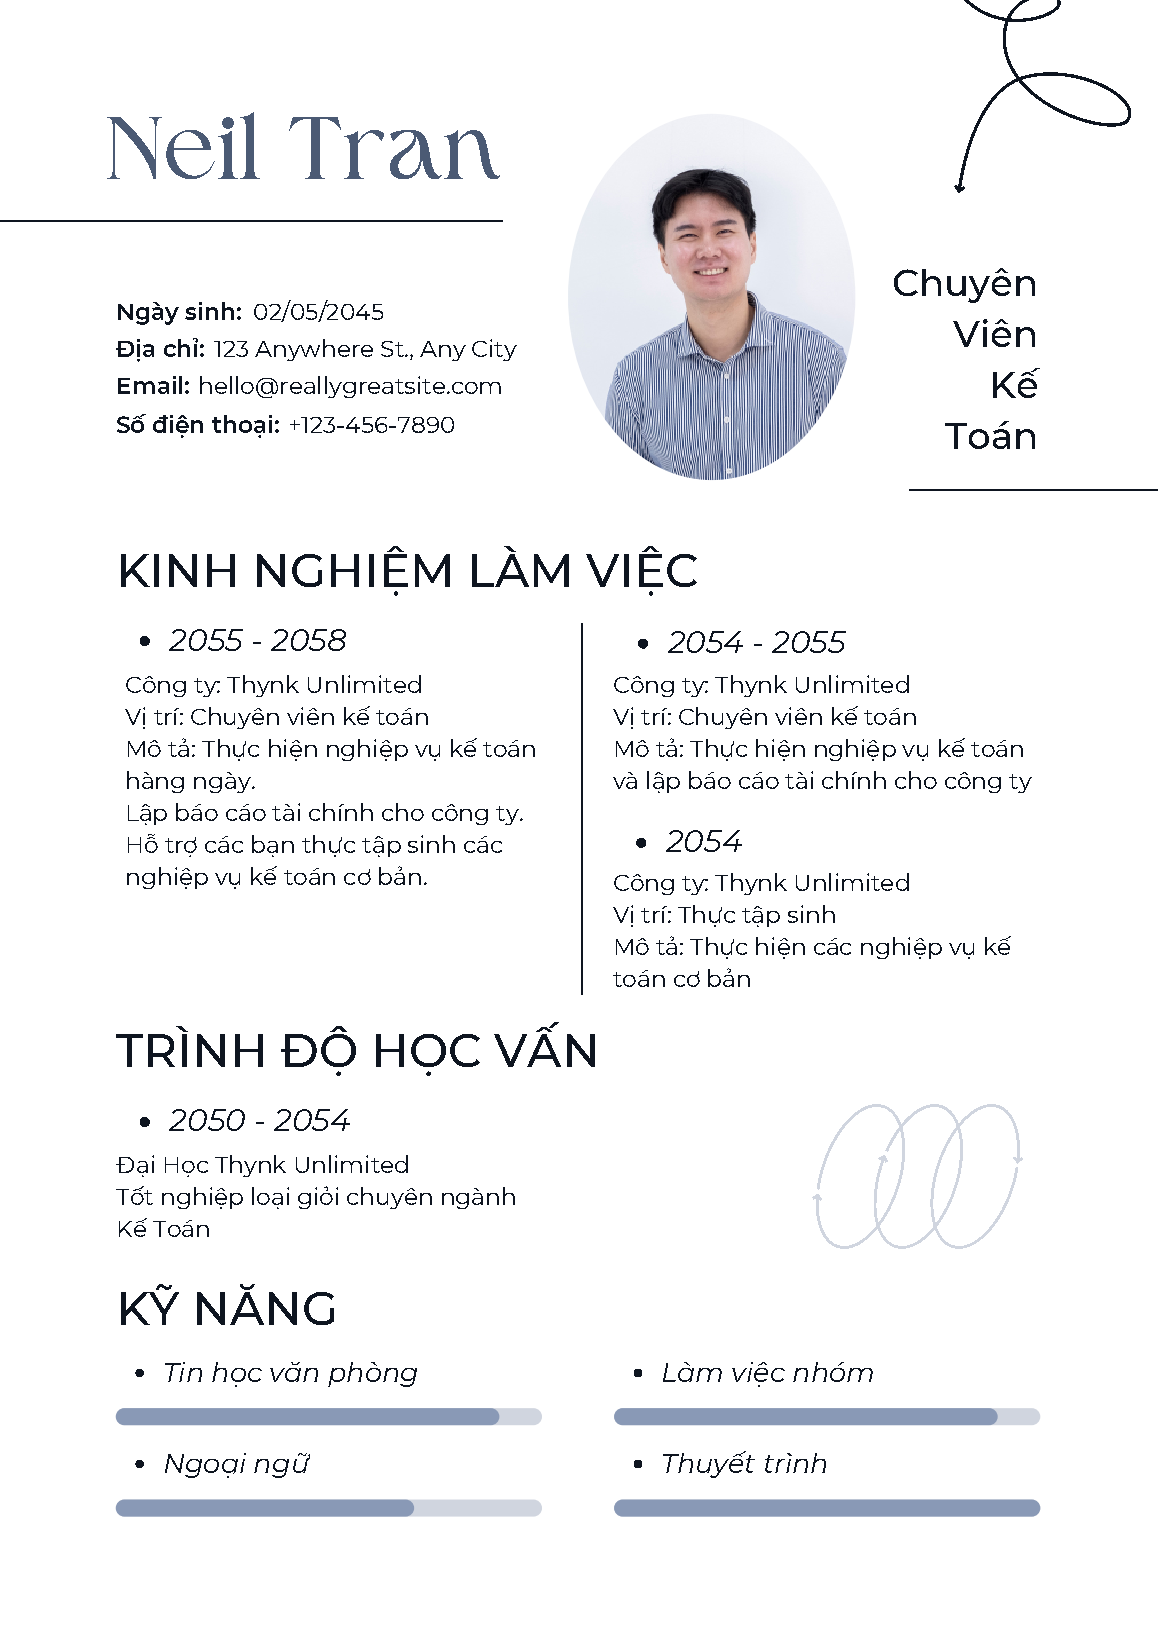
\includegraphics[width=0.66\textwidth]{hinh/cv-review.png}
\caption{Giao diện xem lại hồ sơ CV minh họa sau khi trích xuất.}
\label{fig:cvreview}
\end{figure}

\section{Kiểm thử}
Kho mã có các bộ kiểm tra cho bộ phân tích CV, thành phần cốt lõi, pipeline huấn luyện và dịch vụ embedding. Báo cáo này chưa ghi nhận một lần chạy kiểm thử cuối trên môi trường nộp; cần chạy lại và bổ sung phiên bản runtime, lệnh, số ca đạt/thất bại và lỗi còn tồn tại. Không kết luận toàn bộ kiểm thử đạt khi chưa có log xác nhận.

\chapter{Kết quả và đánh giá}
\label{ch:ketqua}

\begin{muctieu}
Chương này báo cáo kết quả thực nghiệm hiện có, so sánh baseline và phân tích giới hạn của dữ liệu, mô hình và bộ đọc CV.
\end{muctieu}

\section{Kết quả đạt được}
Đồ án đã có ứng dụng web quản lý vị trí tuyển dụng, hồ sơ ứng viên, CV và kết quả matching; backend cung cấp API và cơ chế trích xuất PDF/DOCX; điểm so khớp kết hợp một số tiêu chí và có pipeline huấn luyện Random Forest. Kết quả này đáp ứng mục tiêu xây dựng nguyên mẫu tích hợp. Độ tin cậy trích xuất và mức độ hữu ích trong quy trình tuyển dụng thực tế chưa được đánh giá bằng thử nghiệm người dùng có kiểm soát.

\section{Độ đo đánh giá}
Bảng~\ref{tab:ketqua} ghi lại kết quả trên tập kiểm thử gồm 13.928 bản ghi. Baseline dự đoán lớp đa số đạt accuracy cao hơn mô hình, trong khi Random Forest có macro F1 cao hơn.

\begin{table}[H]
\centering
\caption{So sánh Random Forest với baseline lớp đa số trên tập kiểm thử.}
\label{tab:ketqua}
\begin{tabular}{lcc}
\toprule
\textbf{Chỉ số} & \textbf{Random Forest} & \textbf{Baseline} \\
\midrule
Accuracy & 0,7128 & 0,7434 \\
Macro precision & 0,5422 & -- \\
Macro recall & 0,6148 & -- \\
Macro F1 & 0,5645 & 0,2843 \\
Weighted F1 & 0,7344 & 0,6340 \\
\bottomrule
\end{tabular}
\end{table}

Ma trận nhầm lẫn theo thứ tự nhãn HIGH, MEDIUM, LOW được ghi ở Bảng~\ref{tab:confusion}.
\begin{table}[H]
\centering
\caption{Ma trận nhầm lẫn của Random Forest theo thứ tự HIGH, MEDIUM, LOW.}
\label{tab:confusion}
\begin{tabular}{lrrr}
\toprule
 & \textbf{Dự đoán HIGH} & \textbf{Dự đoán MEDIUM} & \textbf{Dự đoán LOW} \\
\midrule
Thực tế HIGH & 593 & 326 & 111 \\
Thực tế MEDIUM & 612 & 1.238 & 694 \\
Thực tế LOW & 540 & 1.717 & 8.097 \\
\bottomrule
\end{tabular}
\end{table}

\section{Bàn luận}
Accuracy của Random Forest thấp hơn baseline lớp đa số 0,0306, nhưng macro F1 cao hơn 0,2802. Đây là dấu hiệu mô hình cân bằng hơn giữa các lớp theo macro F1, song các số tổng hợp chưa đủ để chứng minh khả năng sàng lọc ứng viên có giá trị thực tế. Lớp LOW có nhiều mẫu hơn các lớp còn lại; vì vậy accuracy của baseline cao dù baseline không phân biệt được từng mức phù hợp.

Lần đánh giá ghi nhận semantic model không khả dụng, nên kết quả không bao gồm tín hiệu embedding ngữ nghĩa. Việc chia dữ liệu theo ứng viên giúp hạn chế rò rỉ cùng hồ sơ giữa các tập, nhưng mô tả công việc lặp lại có thể xuất hiện ở nhiều tập. Dữ liệu chứa bản ghi tổng hợp và nhãn có hỗ trợ bằng mô hình, không phải benchmark độc lập được gán nhãn thủ công.

\section{Hạn chế}
\begin{itemize}[leftmargin=1.6em,itemsep=2pt]
  \item Cần đánh giá trên dữ liệu thật có sự đồng ý và nhãn được chuyên gia xác minh độc lập.
  \item OCR có thể sai với ảnh mờ, bố cục nhiều cột hoặc thiếu gói ngôn ngữ.
  \item Bộ nhận diện trường có thể nhầm mốc thời gian học vấn và thời gian kinh nghiệm; cần kiểm tra CV gốc.
  \item Một số thành phần matching dựa trên quy tắc/từ khóa nên có thể bỏ sót cách diễn đạt tương đương.
  \item Chưa có đánh giá độ chính xác từng trường, độ ổn định theo nhóm ứng viên hoặc thử nghiệm người dùng.
  \item CV chứa dữ liệu cá nhân; cần kiểm soát quyền truy cập, mục đích xử lý và thời hạn lưu.
\end{itemize}

Điểm số chỉ nên hỗ trợ rà soát hồ sơ và không nên là căn cứ duy nhất để loại ứng viên. Các hệ thống tuyển dụng thuật toán cần được xem xét cả về thiên lệch và tác động lên ứng viên~\cite{Fabris2025}.

\chapter{Kết luận và hướng phát triển}
\label{ch:ketluan}

\begin{muctieu}
Chương này tổng kết nguyên mẫu đã xây dựng, nêu giới hạn và các bước phát triển tiếp theo.
\end{muctieu}

\section{Kết luận}
Đồ án xây dựng nguyên mẫu trợ lý tuyển dụng gồm giao diện quản lý, API backend, lưu dữ liệu, đọc CV và tính điểm so khớp. Hệ thống kết hợp các quy tắc trích xuất, độ tương đồng văn bản và mô hình Random Forest. Trên tập đánh giá hiện có, macro F1 của Random Forest cao hơn baseline lớp đa số, trong khi accuracy thấp hơn. Do dữ liệu đánh giá có thành phần tổng hợp và nhãn hỗ trợ bằng mô hình, chưa thể kết luận hiệu quả trên quy trình tuyển dụng thực tế.

\section{Bài học rút ra}
Chất lượng dữ liệu, nhãn và ngữ cảnh hồ sơ ảnh hưởng trực tiếp đến kết quả. Chỉ số tổng hợp không thay thế việc kiểm tra lỗi từng lớp và từng trường trích xuất. Hệ thống AI trong tuyển dụng cần cho phép con người rà soát, giải thích được tín hiệu chính và tránh tự động hóa quyết định bất lợi cho ứng viên.

\section{Hướng phát triển}
\begin{itemize}[leftmargin=1.6em,itemsep=2pt]
  \item Thu thập dữ liệu có sự đồng ý và xây dựng tập nhãn độc lập, có quy trình kiểm tra chất lượng.
  \item Đánh giá riêng độ chính xác trích xuất email, kỹ năng, học vấn và khoảng thời gian kinh nghiệm.
  \item Cải thiện phân đoạn bố cục và nhận diện ngữ cảnh thời gian để giảm nhầm lẫn giữa học vấn và kinh nghiệm.
  \item Kiểm tra thiên lệch theo nhóm phù hợp với quy định và dữ liệu có thể sử dụng; lưu giải thích các thành phần điểm.
  \item Hoàn thiện kiểm thử tích hợp, bảo vệ dữ liệu cá nhân và đánh giá với người dùng tuyển dụng.
\end{itemize}

\backmatter
\cleardoublepage
\phantomsection
\addcontentsline{toc}{chapter}{Tài liệu tham khảo}
\bibliographystyle{plain}
\bibliography{refs}
\chapter{Phụ lục}
\markboth{Phụ lục}{}

\section*{A. Hướng dẫn cài đặt và chạy chương trình}
\phantomsection
\addcontentsline{toc}{section}{A. Hướng dẫn cài đặt và chạy chương trình}

Các bước sau được lấy từ README của dự án. Cần chạy thử trên máy dùng để bảo vệ trước khi nộp.

\begin{lstlisting}[language=bash,caption={Khởi chạy ứng dụng bằng Docker Compose.}]
# In the project root
 docker compose up --build

# Open the web application
 http://localhost:5173

# Open the FastAPI documentation
 http://localhost:8000/docs
\end{lstlisting}

\section*{B. Bảng tự kiểm trước khi nộp}
\phantomsection
\addcontentsline{toc}{section}{B. Bảng tự kiểm trước khi nộp}

\begin{tukiem}
  \item Đã thay thông tin sinh viên và giảng viên trên trang bìa.
  \item Đã đọc, xác nhận và ký lời cam đoan; đã cá nhân hóa lời cảm ơn.
  \item Đã chạy ứng dụng và kiểm thử trên đúng môi trường bảo vệ.
  \item Đã kiểm tra các con số trong báo cáo với log huấn luyện cuối.
  \item Mọi tài liệu tham khảo trong danh mục đều được trích dẫn trong nội dung.
  \item Đã kiểm tra quyền sử dụng dữ liệu, hình ảnh và tệp CV minh họa.
  \item Đã giải thích trong báo cáo phần sử dụng công cụ AI hỗ trợ theo quy định học phần.
  \item Đã kiểm tra PDF cuối, hình/bảng, mục lục và không còn nội dung mẫu.
\end{tukiem}

\end{document}


